\documentclass[12pt, letterpaper]{article}
\usepackage{color}
\usepackage{natbib}
\usepackage{parskip}
\usepackage{amsmath}
\usepackage{amssymb}
\usepackage{wrapfig}
\usepackage{graphicx}
\usepackage{listings}
\usepackage{setspace}
\usepackage{geometry}
\usepackage{enumitem}
\usepackage{dirtytalk}
\usepackage{subcaption}
\usepackage{indentfirst}
\usepackage{anyfontsize}
\usepackage[utf8]{inputenc}

\parindent=0.5in

\graphicspath{{./imgs/}}

\definecolor{codegray}{rgb}{0.2,0.2,0.2}
\definecolor{codepurple}{rgb}{0.58,0,0.82}
\definecolor{backcolor}{rgb}{0.95,0.95,0.92}

\newcommand{\sorta}[1]{\lq #1\rq \,}

\lstdefinestyle{scheme}
  {backgroundcolor=\color{backcolor},
  commentstyle=\color{blue},
  keywordstyle=\color{magenta},
  numberstyle=\tiny\color{codegray},
  stringstyle=\color{codepurple},
  basicstyle=\footnotesize\ttfamily,
  morekeywords={*},
  breakatwhitespace=false,
  breaklines=true,
  captionpos=t,
  keepspaces=true,
  numbers=left,
  numbersep=5pt,
  showspaces=false,
  showstringspaces=false,
  showtabs=false,
  tabsize=2,
  title=\lstname,
  language=Python
}

\lstset{style=scheme}

\doublespace{}
\title{On Splines and Their Use in Computer Graphics and Generating Curves}
\author{Simon Abrelat}
\date{\vspace{-5ex}}

\DeclareUnicodeCharacter{2212}{-}
\begin{document}

\large
{\fontsize{12}{14.4}
  {\singlespace{}
  \pagenumbering{gobble}
  \maketitle
  \begin{center}
  \vspace{4mm}
  002129--0004 \\
  \vspace{4mm}
  Math HL IA \\
  \vspace{4mm}
  May 2019 \\
  \vspace{4mm}
  Words: \\
  \end{center}
  }
}
\newpage

\pagenumbering{arabic}
\begin{abstract}
Splines are used everywhere around us, from fonts to animations. They are the way that computers manipulate
and store curves, and because of that have a large range of possible applications. Since they are so useful, 
there are also
many of ways to generate these functions and lots of formats they come in. In general, they are fairly
computationally cheap which makes them so applicable and expendable. This paper will illustrate and help
visualize different types of splines.
\end{abstract}

\newpage
\tableofcontents
\newpage

\section{Introduction}
Splines are not a specific equation. They are more a class of equations that have similar properties. They 
are simply piecewise polynomials, and are often parameterized so that they can \sorta{loop over themselves}
and break the vertical line test. One of the interesting aspects of splines is that they keep this
property even at low degrees.


The word spline is derived from wooden splines that curve and are often
used in things like braces for ships. The major benefit of splines is how they are suited for computers.
Almost all curves on a computer, from fonts to animation paths, are described quickly and accurately by
splines such as B\`ezier and Hermite curves. This means that these splines are around us all of the time and 
are almost invisible if you do not know where to look. There are many different kinds of splines with
different methods of formulation. However, this paper will primarily focus on Hermite and B\`{e}zier curves.

\section{B\`ezier Curves}
\subsection{Theory}
B\`ezier curves can be made with a linear combination of Bernstein polynomials \citep{ams}. Bernstein
polynomials were first used in the proof of the Stone-Weierstrass theorem which states that every continuous
function defined on a closed interval $[a,b]$ can be approximated as closely as desired by a polynomial
\citep{weierstrass}. This means that a Bernstein polynomial can make any other function as the degree
approaches infinity (\ref{eq:BLimit}) A Bernstein polynomial (\ref{eq:BPoly}) is defined by a linear combination of Bernstein
basis functions (\ref{eq:BBasis}).

Bernstein Polynomials:
\begin{singlespace}
  \begin{equation}
    \label{eq:BBasis}
    b_{\nu,n}(t) = {n \choose \nu} t^\nu (1 - t)^{n - \nu}
  \end{equation}
  \begin{equation}
    \label{eq:BPoly}
    B_n(t) = \sum_{\nu = 0}^{n}\beta_\nu b_{\nu,n} (t)
  \end{equation}
  \begin{small}  
    \begin{itemize}[label=]
      \item $\beta_\nu$: the control point component
    \end{itemize}
  \end{small}
  \begin{equation}
    \label{eq:BLimit}
    \lim_{n\to\infty} B_n(f) = f
  \end{equation}
  \begin{small}
		\begin{itemize}[label=]
    	\item $n$: degree of the Bernstein function
    	\item $\nu$: number of the $n+1$ equations of a function of degree $n$ 
		\end{itemize}
  \end{small}
\end{singlespace}

\begin{figure}[ht]
  \caption{Basis functions for different degrees, Listing~\ref{lst:BBasis}}
  \label{fig:basis}
  \begin{center}
    \begin{subfigure}[b]{.45\linewidth}
      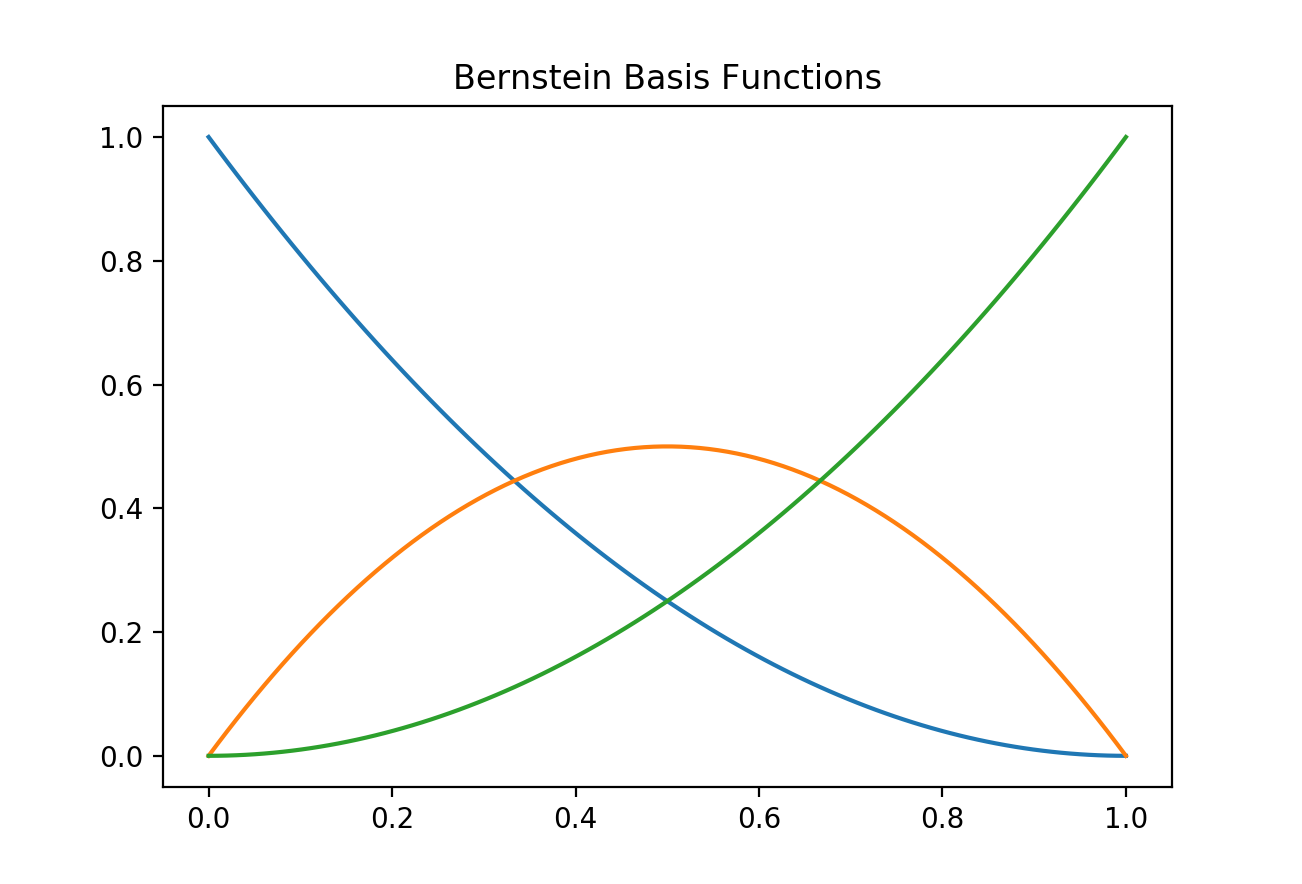
\includegraphics[width=\linewidth]{Basis/basis2}
      \caption{$n=2$}
    \end{subfigure}
    \begin{subfigure}[b]{.45\linewidth}
      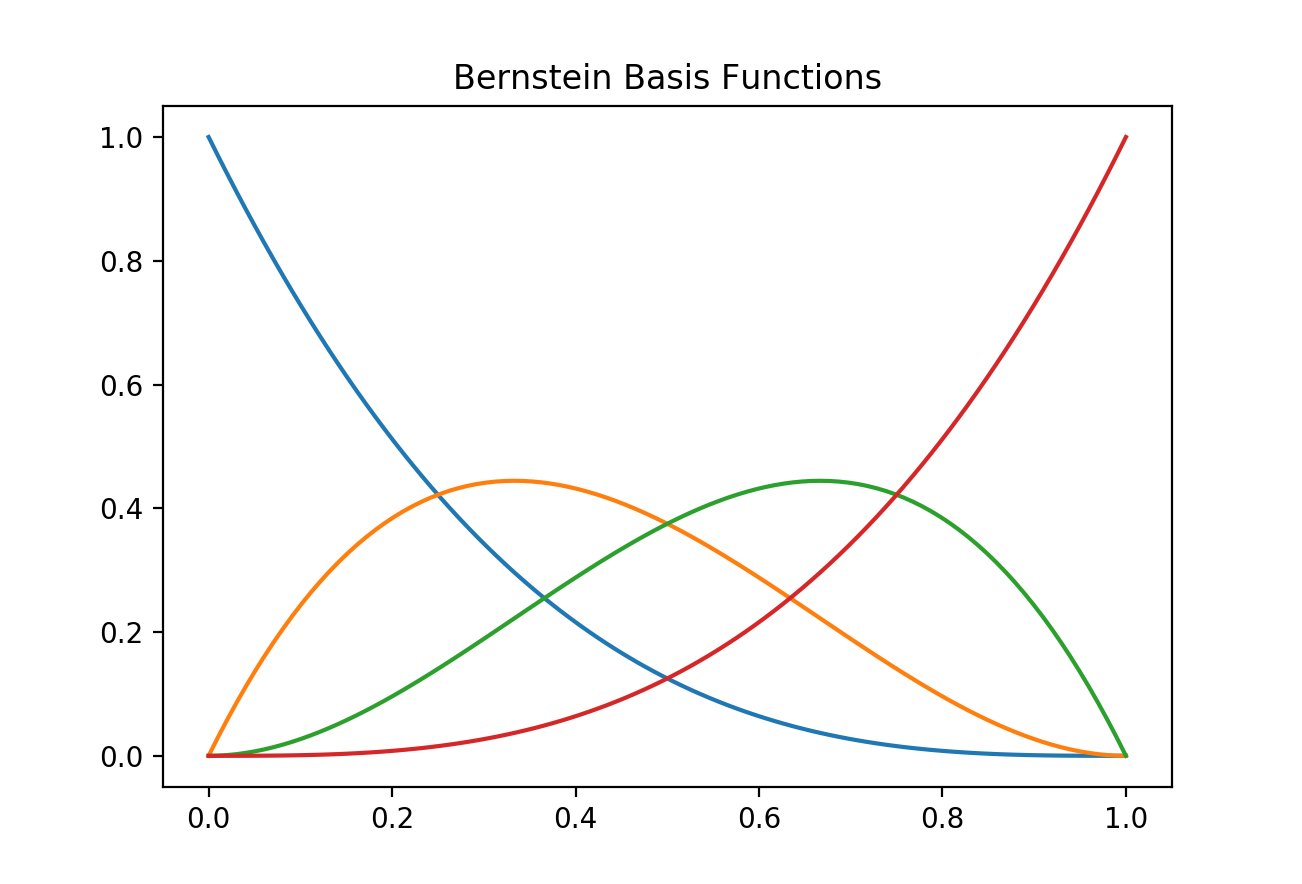
\includegraphics[width=\linewidth]{Basis/basis3}
      \caption{$n=3$}
    \end{subfigure}
  \end{center}
\end{figure}
\begin{figure}[ht]
  \begin{center}
    \begin{subfigure}[b]{.45\linewidth}
      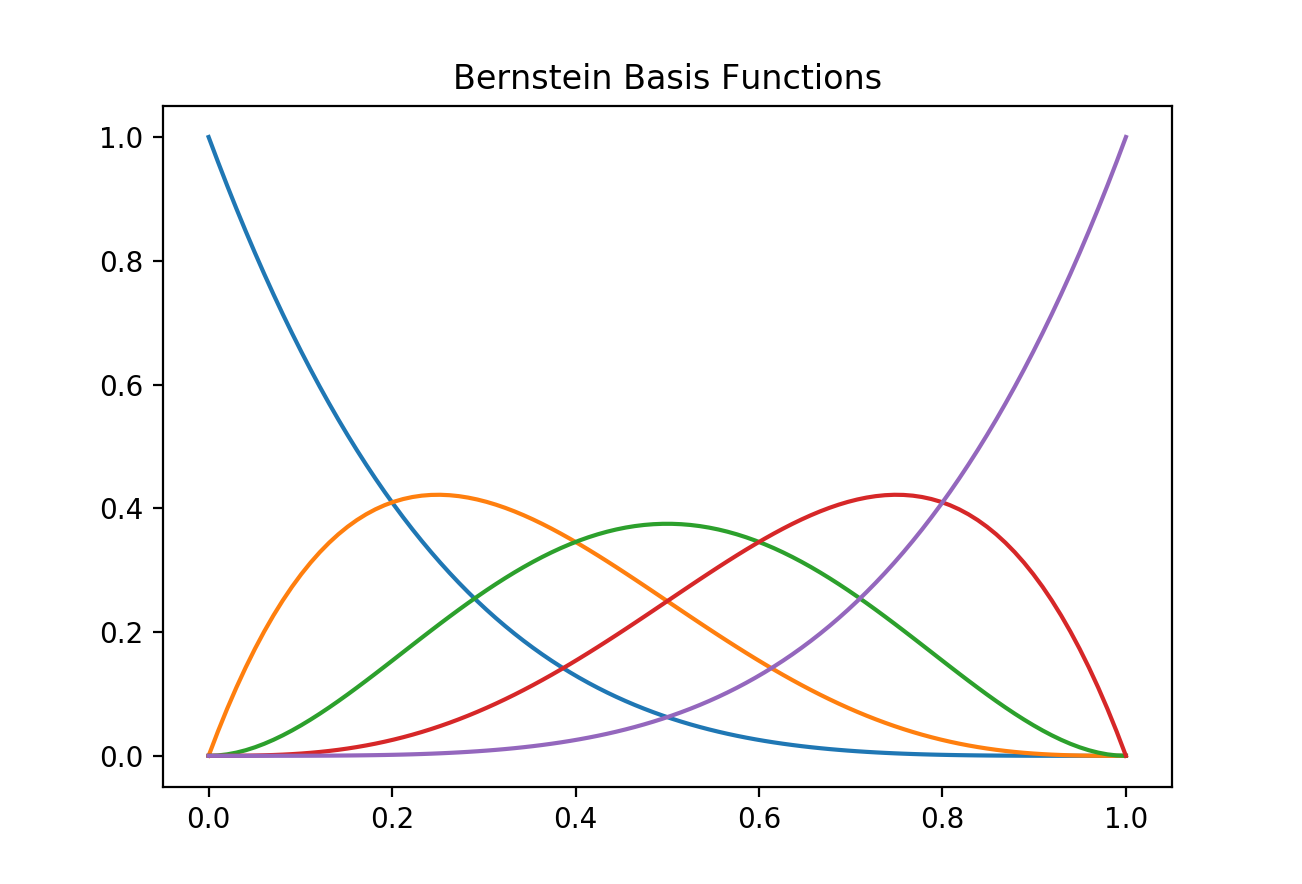
\includegraphics[width=\linewidth]{Basis/basis4}
      \caption{$n=4$}
    \end{subfigure}
    \begin{subfigure}[b]{.45\linewidth}
      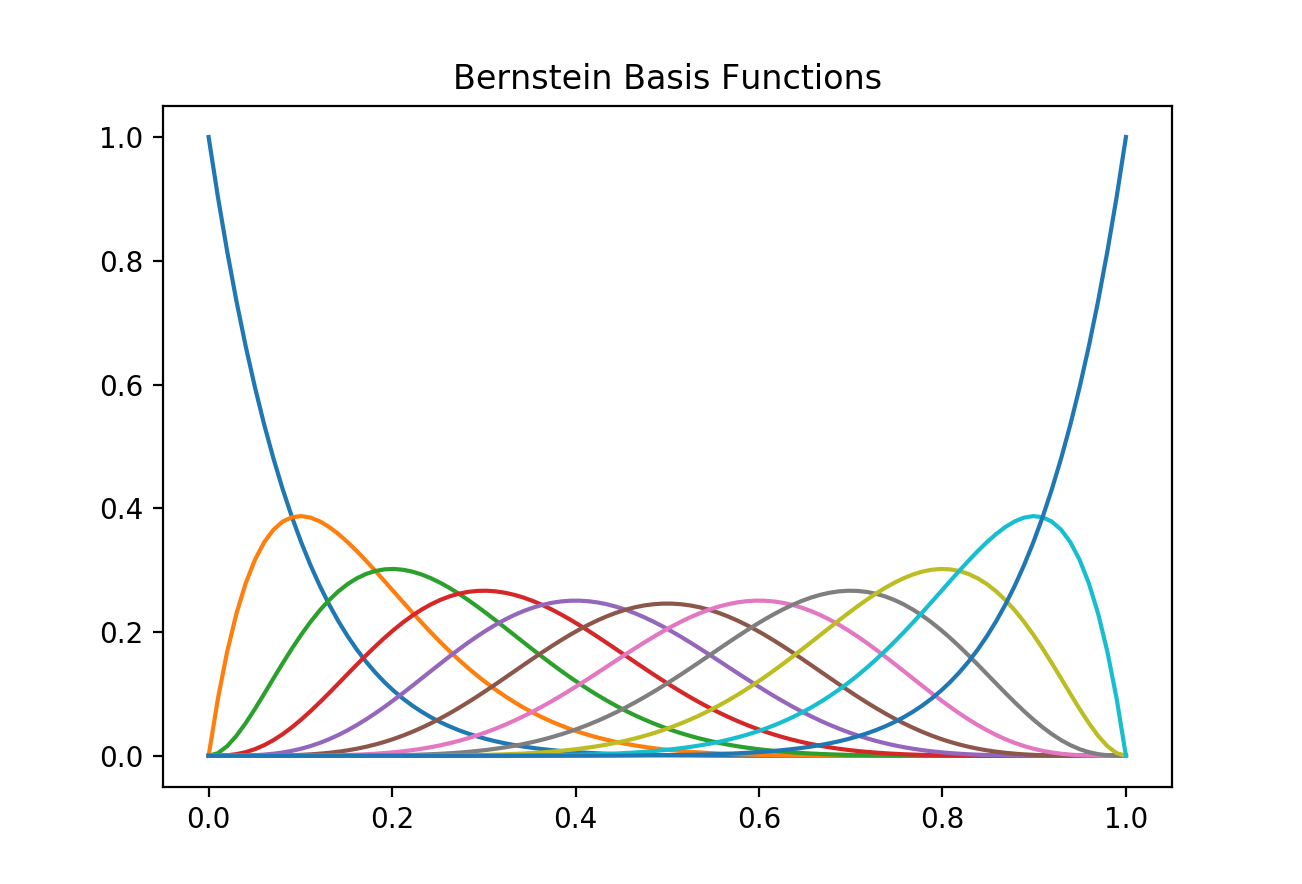
\includegraphics[width=\linewidth]{Basis/basis10}
      \caption{$n=10$}
    \end{subfigure}
  \end{center}
\end{figure}

Bernstein functions are only approximations and to perfectly match the original function you would need an 
infinite degree Bernstein polynomials, similar to Taylor series (\ref{eq:BLimit}). The algorithm used to
generate a B\'ezier curve given a set of control points is called De Castlejau's algorithm. It is a recursive
algorithm (\ref{eq:DCRec}) that takes control points and interpolates a curve between them. This method is a
little more complicated than the explicit form (\ref{eq:DCExplicit}) which is a summation of the control
points multiplied by the basis functions of a given degree $n$. Then to generate any possible curve, 
parameterize the $x$ and $y$ axes and fun De Castlejau's algorithm on the scalar $x$ and $y$ quantities. 

\begin{singlespace}
  \begin{gather}
    \label{eq:DCRec}
    \beta_{1}^{(0)} = \beta_i \quad i = 0,\ldots, n \\
    \beta_{i}^{(j)} = \beta_{\nu}^{(j-1)} (1 - t_0) + \beta_{\nu}^{(j-1)} t_0
  \end{gather}
  \begin{small}
    \begin{itemize}[label=]
      \item $j$ = $1,\ldots,n$
      \item $\nu$ = $0,\ldots,n-j$
    \end{itemize}
  \end{small}
  \begin{equation}
    \label{eq:DCExplicit}
    B(t) = \sum_{\nu=0}^{n} \beta_\nu b_{\nu,n}(t)
  \end{equation}
  \begin{small}
    \begin{itemize}[label=]
      \item $\beta_\nu$: $i$th control point
      \item $b_{\nu,n}(t)$: Bernstein basis function for the number and degree
    \end{itemize}
  \end{small}
\end{singlespace}

\subsection{Application}
There are practically an infinite number of uses for B\`ezier curves. They, and other similar methods, are 
used
to display all curves in computers which means that anything made graphically with curves use B\`ezier curves
or similar splines. However, the hidden ubiquitous use of B\`ezier curves in particular is in 
fonts. All PostScript fonts, the basis of PDFs, use cubic B\`ezier curves (a) and TrueType fonts,
abbreviated to ttf, use quadratic B\`ezier curves (b).

\begin{figure}[ht]
  \label{fig:BezierCurves1}
  \caption{Cubic and Quadratic Curves, Listing~\ref{lst:bez}}
  \begin{center}
    \begin{subfigure}[b]{.45\linewidth}
      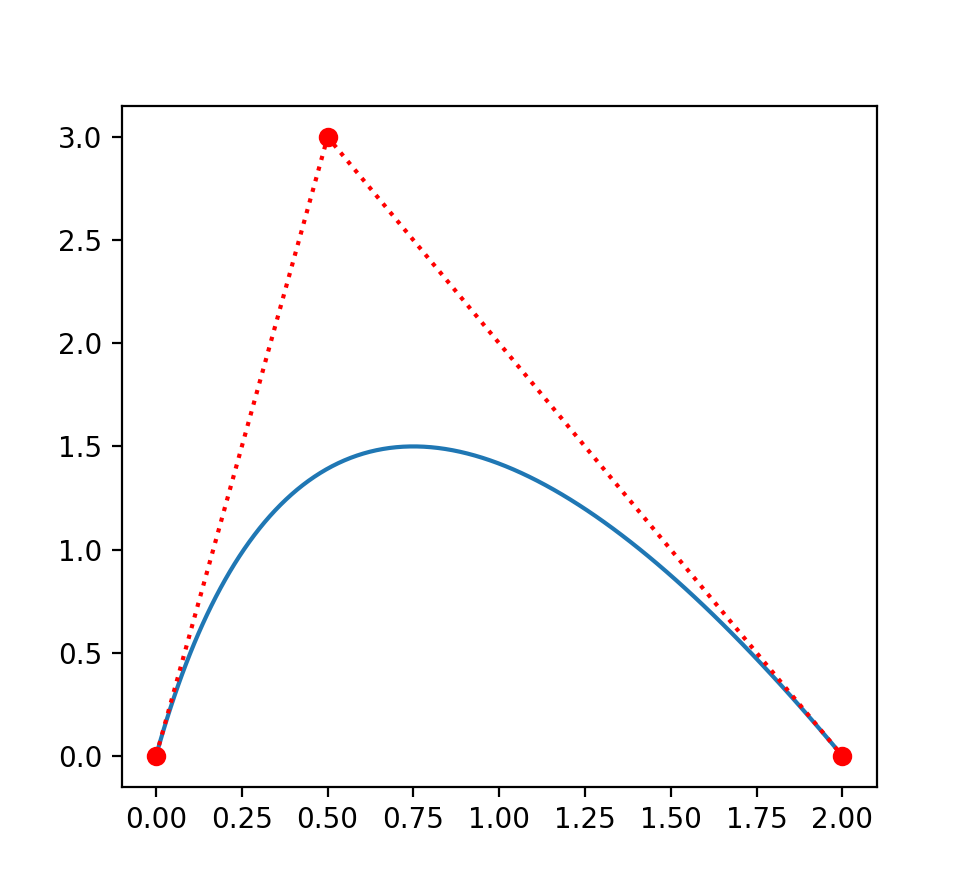
\includegraphics[width=\linewidth]{Bez/cubicBez1}
      \caption{Cubic curve, 3 control points}
    \end{subfigure}
    \begin{subfigure}[b]{.45\linewidth}
      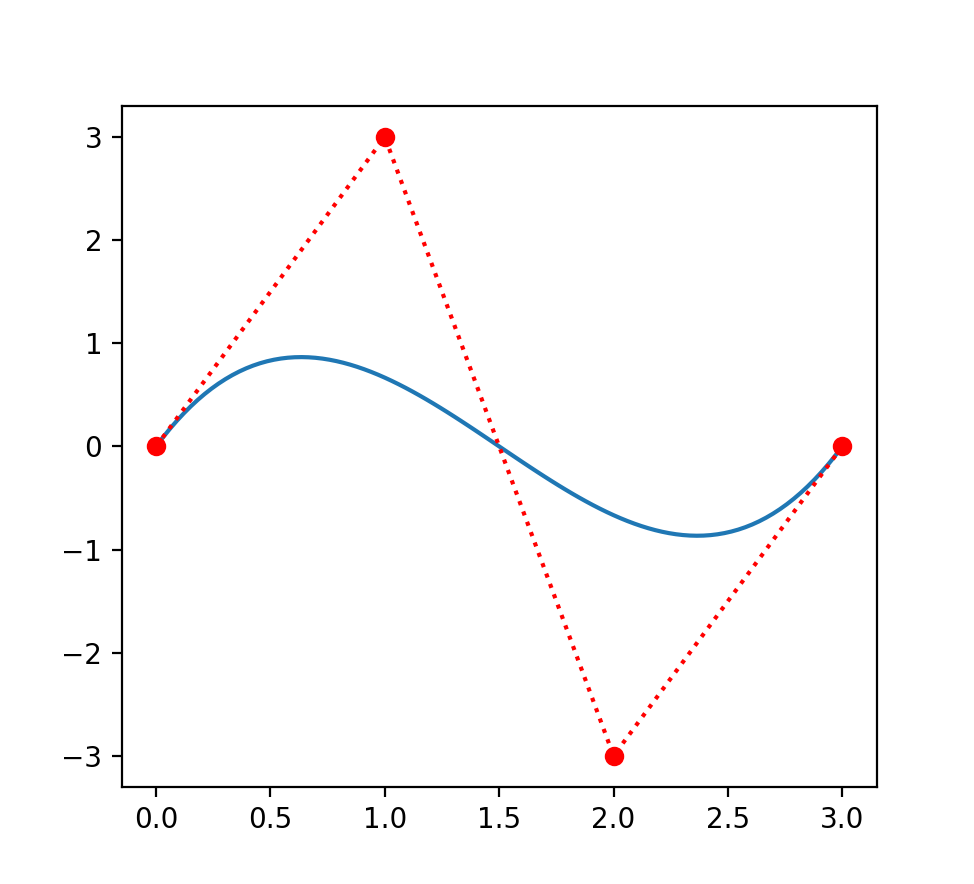
\includegraphics[width=\linewidth]{Bez/quadraticBez1} \caption{Quadratic curve, 4 control points}
    \end{subfigure}
  \end{center}
\end{figure}

Most of the computer generated graphics, such as advertisements, animations, icons contain B\`ezier curves.
The popular software used for graphic design is Adobe Illustrator\textsuperscript\textregistered \, which is 
a vector graphics editor that is entirely based on manipulating B\`ezier curves.
It generates curves with specific parameters being 2 anchor and 2 control points which is exactly the
quadratic B\`ezier curve. 

The other uses for B\`ezier curves are in optimization problems. Since they are used to approximate a 
curve, and the control point can be related to the derivative of a function, they are very useful for
optimization problems. They can be used to minimize path lengths \citep{bezierPaths} and can even have
restrictions such as a maximum acceleration or velocity \citep{bezierSoccerPaths}. The acceleration and
velocity limits are caused by the control points which can be controlled since they are tangential to
their anchor points meaning the angle is related to the derivative of the function and the magnitude of
the control point is related to the acceleration or multiple control points. These values can even be 
used to model resistance in a parameterized manner so yet another use of B\`ezier curves would be the
generation of an optimal airfoil \citep{bezierAirfoil}.

\section{Hermite}

\subsection{Theory}


A cubic Hermite spline takes two control points and the derivatives. There are also higher order Hermite
splines such as quintic splines that take 2 points their derivatives as well as their second derivatives. For
this section, however, we will be focusing on cubic splines. These cubic splines have 4 basis functions much
like the Bernstein basis functions for B\`ezier curves. In fact, you can express Hermite basis functions in
terms of their Bernstein counterparts (equation~\ref{eq:BBasis}); however, a linear combination of Bernstein
Basis functions approximates any polynomial. Two of those functions are for the points and then there are 2 
for the derivatives.

\begin{figure}[!h]
  \centering
  \caption{Hermite Bases, Listing~\ref{lst:HBasis}}
  \label{fig:HBasisGraphs}
  \includegraphics[width=.3\linewidth]{Basis/HBasis}
  \vspace{-10pt}
\end{figure}
\begin{singlespace}
  \begin{equation}
    \begin{aligned}
      &h_{0,0}(t) = (1+2t)(1-t)^2 &&= \beta_0(t) + \beta_1(t) \\
      &h_{1,0}(t) = t(1-t)^2 &&= \frac{\beta_1(t)}{3}\\
      &h_{0,1}(t) = t^2(3-2t) &&= \beta_2(t) + \beta_3(t)\\
      &h_{1,1}(t) = t^2(1-t) &&= \frac{-\beta_2(t)}{3}
    \end{aligned}
  \end{equation}
  \begin{small}
  i  \begin{itemize}[label=]
      \item $h_{0,0}$: is function for the first point
      \item $h_{0,1}$: is function for the first derivative
      \item $h_{1,0}$: is function for the second point
      \item $h_{1,1}$: is function for the second derivative
      \item $\beta_n$: Bernstein basis function with degree 3 for index $n$
    \end{itemize}
  \end{small}
\end{singlespace}


Another way to describe Hermite splines, as well as B\`ezier curves, is through matrices (\ref{eq:HMatrix}).
These matrices are equivalent to the basis functions. The benefit of using matrices is that it is easier to
change between different types of splines for different purposes. For example, if one were making a
application they could pass in the basis matrix to generate Hermite, B\`ezier, Catmull-Rom, or other forms.

\begin{figure}[h!]
  \centering
  \caption{1D Hermite Interpolation, Listing~\ref{lst:hermite}}
  \label{fig:HermiteGraph}
  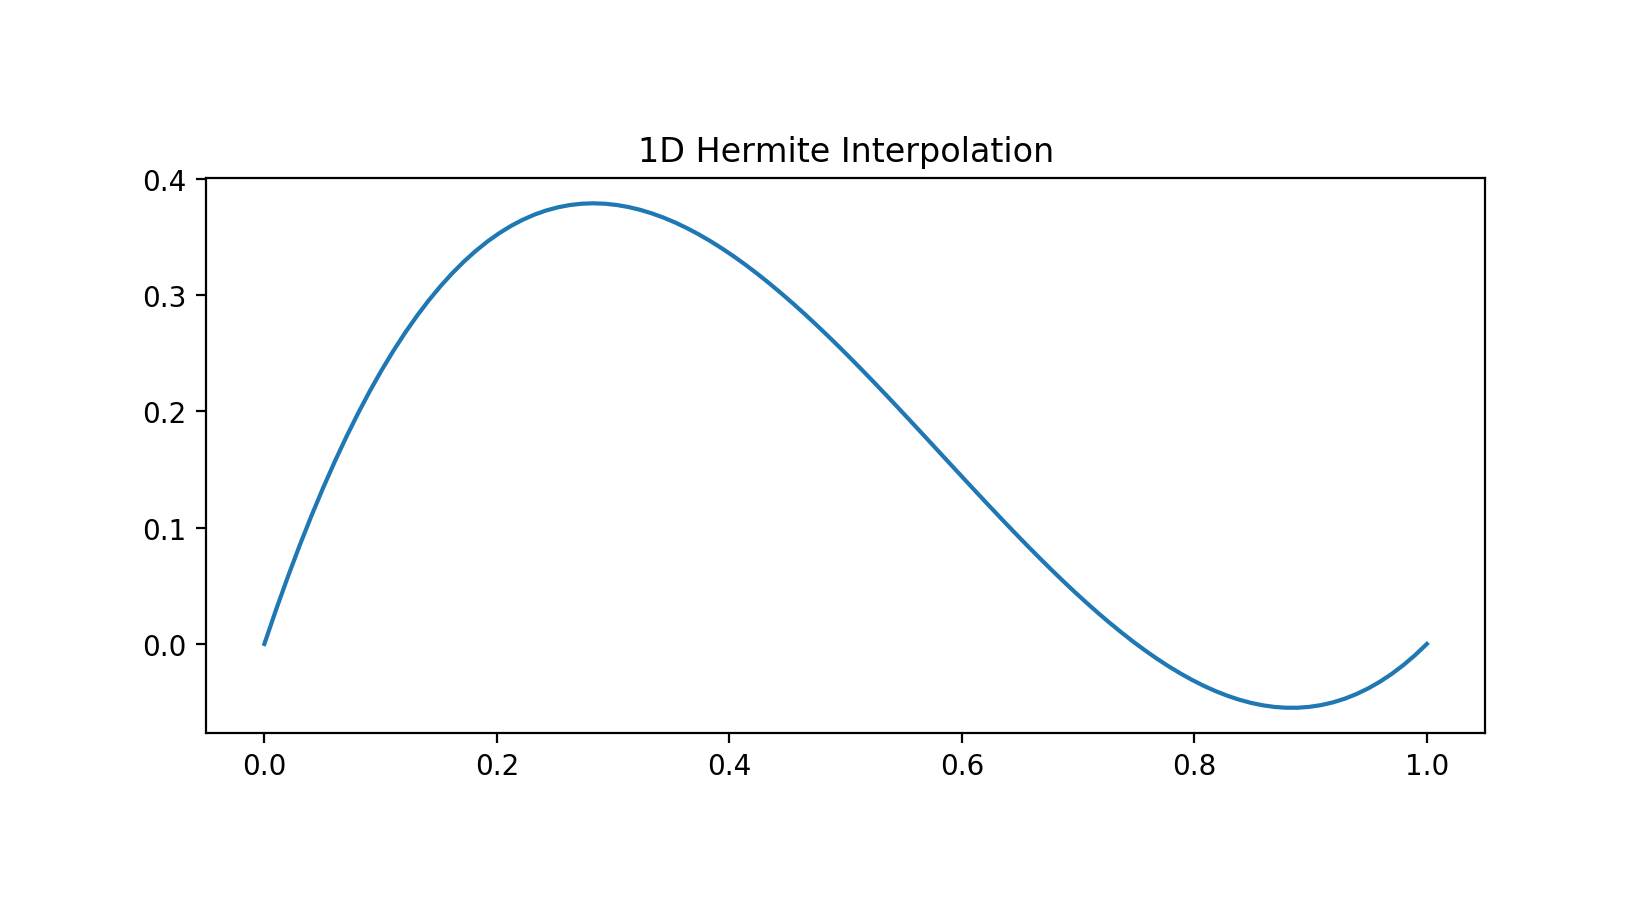
\includegraphics[width=\linewidth]{hermite1}
  \vspace{-10pt}
\end{figure}

\begin{equation}
  \label{eq:HMatrix}
  p = 
  \begin{bmatrix}
    s^3 & s^2 & s & 1
  \end{bmatrix}
  \begin{bmatrix}
     2 & -2 &  1 &  1 \\
    -3 &  3 & -2 & -1 \\
     0 &  0 &  1 &  0 \\
     1 &  0 &  0 &  0
  \end{bmatrix}
  \begin{bmatrix}
    p_{n-1} \\
    p \\
    p_{n+1} \\
    p_{n+2}
  \end{bmatrix}
\end{equation}

\subsection{Application}
Interpolated splines are useful for a host of different applications. Hermite splines
are not as ubiquitous, but they have more specific uses. They are often used for statistics since they can
generate intermediate values between data points as well as being used for regression and filtering
\citep{HRegression}. Hermite splines are also used for path generation for simple mobile or differential
robots. In the study \cite{HMove}, they use genetic algorithms to optimize Hermite paths to simulate
bipedal, tripedal, and \sorta{snake-like} motion. 

\begin{figure}[ht]
  \centering
  \caption{The different Types of Wavelets}
  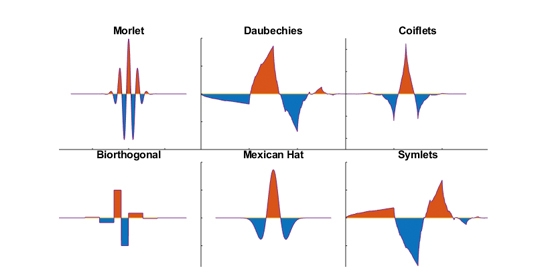
\includegraphics[width=\linewidth]{wavelets}
  \label{fig:waveletFig}
\end{figure}

One of the biggest uses of Hermite splines are wavelets \citep{HWavelets}. These are wavelets and not waves
since they terminate and do not oscillate to infinity (figure~\ref{fig:waveletFig}). In signals processing,
Fourier Transforms isolate the frequency and amplitude of a signal which includes all of the image. Wavelets
allow one to find the local transformations such as edges or lines in an image. Most of the purely academic
uses of
Hermite splines are in modeling different forms of wavelets or other signal analysis. For example, in
\cite{HBioMed} they are using wavelets for edge detection as well as for modeling the blobs, or objects that
make edges, to automatically analyze medical photos. As previously alluded to, these interpolating
splines can be used for smoothing or filtering data. Hermite splines can also be used for interpolation
between data points which can be used for filtering. So for the application of signals processing, splines
can be used for generating data and cleaning it up.

\section{Conclusion}
B\`ezier and Hermite splines are just two examples in a sea of possible splines. These are two simple types
that are useful for outlining the two archetypes of splines, interpolating and weighted, while still being
computationally simple. However, their simplicity does not subtract from their functionality or abundance in
real life applications. There are often \sorta{better} or more specialized splines for any given use case;
however, that misses the point of their power and generality. The naively simple task of making an
approximation of curve between points has much more depth than one can possibly cover. The simplicity and
generality also explains why splines are everywhere.

\newpage
\bibliographystyle{apa}
\bibliography{IA}
\newpage
\section{Appendix}
\listoffigures

\lstinputlisting[language=Python, label={lst:BBasis}, caption={Bernstein Basis Functions}]{code/BBasis.py}
\newpage
\lstinputlisting[language=Python, label={lst:bez}, caption={B\`ezier Curves}]{code/bez.py}
\lstinputlisting[language=Python, label={lst:HBasis}, caption={Hermite Basis Functions}]{code/HBasis.py}
\lstinputlisting[language=Python, label={lst:hermite}, caption={Hermite 1D interpolation}]{code/Hermite.py}

\end{document}
